\documentclass[a4paper,12pt,twoside]{article}

\usepackage{graphicx}
\usepackage{amsmath}
\usepackage[english]{babel}
\usepackage[utf8]{inputenc}
\usepackage[colorlinks,bookmarks=false,linkcolor=blue,urlcolor=blue]{hyperref}
\usepackage{color}
\usepackage[T1]{fontenc}
\usepackage{float}
\usepackage{url}
\usepackage{lscape}
\usepackage{tikz}
\usetikzlibrary{patterns,decorations.pathreplacing}
\usepackage[stable]{footmisc}
\usepackage{wrapfig}
\usepackage{textcomp}
\usepackage{changepage}
\usepackage{booktabs}
\usepackage{subfig}
\usepackage{amssymb}
\usepackage[section]{placeins}
\usepackage{mathabx}


\paperheight=297mm
\paperwidth=210mm

\setlength{\textheight}{235mm}
\setlength{\topmargin}{-1.2cm} 
\setlength{\textwidth}{15cm}
\setlength{\oddsidemargin}{0.56cm}
\setlength{\evensidemargin}{0.56cm}

\pagestyle{plain}

% def
\def \be {\begin{equation}}
\def \ee {\end{equation}}
\def \dd  {{\rm d}}
\def \bf {\textbf}
\def \bea {\begin{eqnarray}}
\def \eea {\end{eqnarray}}
\def \bi {\begin{itemize}}
\def \ei {\end{itemize}}
\def \ib {\item[$\bullet$]}
\def \H {{\mathcal H}}
\def \grad{\nabla}
\def \( {\left(}
\def \) {\right)}
\def \order {{\cal O}}



\newcommand{\mail}[1]{{\href{mailto:#1}{#1}}}
\newcommand{\ftplink}[1]{{\href{ftp://#1}{#1}}}
\newcommand{\e}{{\mathrm e}}
\renewcommand{\labelitemii}{$-$}

% ======= Le document commence ici ======

\begin{document}
% Le titre, l'auteur et la date
\title{Project 3 -- Ambient Visualisation of Energy}
\date{\today}
\author{ Giacomo Giudice\\{ \small \mail{giacomog@kth.se}}}
\maketitle

\baselineskip=16pt
\parindent=15pt
\parskip=5pt
\begin{figure}[H]
\centering
{
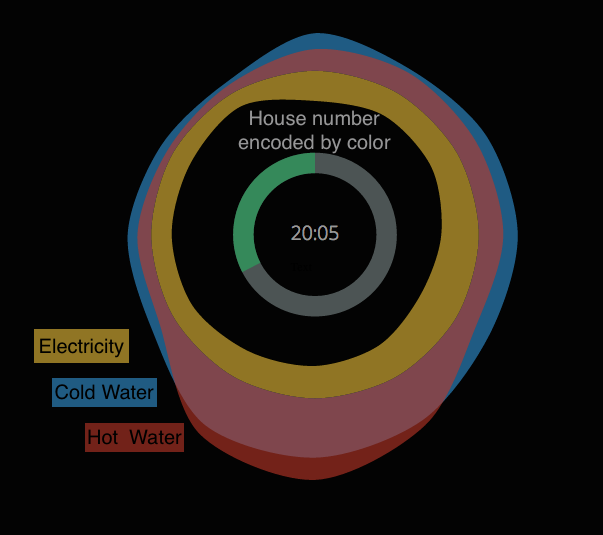
\includegraphics[width=13cm,angle=0]{view.png}
}
\caption{\label{v}}
\end{figure}
\paragraph{Data}
The raw data contained the hourly values (in some unit of measurement) of the following utilities {\em Electricity}, {\em Cold Water}, {\em Hot Water}.
After command line manipulation and some Perl crunching through files (see {\tt raw/sort.pl}), the raw data was processed to have the hourly averages of each utility for each house (see {\tt js/data.js}). 

\paragraph{Design} The main idea is to have a somewhat of a streamgraph around a clock, that shows the household consumptions in 12 hour periods. One conceptual challenge was to  separate the energy and the two different water flows, as they had different units (unless we assume the data is in Planck units, $\hbar = c  = 1$, so mass has the same units as energy). The solution was to keep the energy flow on the inside of the hours circle, and at the same time superpose the water averages on the outside of the hour circle, to promote a visual comparison (see fig.~\ref{v}).

To have a placing of the hours similar to analog clock, that gives an immediate understanding of the time displayed, the visualization was separated in two cycles of twelve hours. Thus, when the clock reaches 12 o'clock, the streamgraph is updated to show the data for the following cycle.
Additionally, after a 24 hour period, the visualization displays the consumptions for the other house.

The interaction is purposely kept at a minimum, as the user is invited to observe the changes in the patterns rather than actively interact with the visualisation.
\paragraph{Further Developments} In this demo the cycle repeats itself in a relatively small amount of time, that it could be made into a video. Another option is to have multiple clocks for each house and instead of displaying averages it could iterate through the daily data and show the consumption day by day. This is less informative at a glance (the averages are of course more meaningful), but would create a very long sequence of different shapes.

\end{document} %%%% THE END %%%%
